% =====================================================================
% Plantilla estándar de figuras de ejercicios — MatePre / Admi-Tec
% =====================================================================
% Uso en Overleaf:
%   1. Proyecto nuevo → pega este archivo como main.tex.
%   2. Dibuja tu figura dentro del tikzpicture (hay un ejemplo abajo).
%   3. Compila → descarga el PDF → conviértelo a SVG con Inkscape,
%      o usa la variante dvisvgm (ver README.md) para SVG directo.
%
% Regla de estilo: TODO se dibuja con los estilos definidos aquí
% (figura / auxiliar / resalte / punto / eje / cota). No inventes
% colores ni grosores nuevos: eso es lo que mantiene las figuras
% consistentes entre ejercicios.
% =====================================================================

\documentclass[tikz, border=4pt]{standalone}
% Para exportar SVG directamente en Overleaf (ver README.md), usa:
% \documentclass[dvisvgm, tikz, border=4pt]{standalone}

\usetikzlibrary{angles, quotes, arrows.meta, calc}

% ---- Paleta (espejo del design system de la app) ------------------
\definecolor{tinta}{HTML}{20242E}   % app-ink: trazos principales y texto
\definecolor{azul}{HTML}{33418F}    % app-primary: marcas secundarias (ángulos, curvas)
\definecolor{ambar}{HTML}{E8A33D}   % app-highlighter: SOLO el elemento que se pregunta
\definecolor{grisaux}{HTML}{9AA0AB} % líneas auxiliares y cotas

% ---- Estilos estándar ----------------------------------------------
\tikzset{
  % Trazo principal: contornos de la figura (triángulo, circunferencia…)
  figura/.style   = {line width=1pt, color=tinta, line cap=round, line join=round},
  % Líneas auxiliares: alturas, prolongaciones, proyecciones
  auxiliar/.style = {line width=0.6pt, color=grisaux, dashed, line cap=round},
  % El elemento que el ejercicio PREGUNTA (uno solo por figura)
  resalte/.style  = {line width=1.2pt, color=ambar, line cap=round},
  relleno resalte/.style = {fill=ambar, fill opacity=0.18, draw=none},
  % Vértices y puntos marcados
  punto/.style    = {circle, fill=tinta, inner sep=0pt, minimum size=3.2pt},
  % Ejes de coordenadas
  eje/.style      = {line width=0.7pt, color=tinta, -{Stealth[length=6pt]}},
  % Cotas de medida (doble flecha)
  cota/.style     = {line width=0.5pt, color=grisaux,
                     {Stealth[length=4pt]}-{Stealth[length=4pt]}},
  % Etiquetas: siempre en modo matemático ($A$, $x$, $8$) — la fuente
  % Computer Modern es la misma familia que usa KaTeX en el enunciado.
  every node/.style = {color=tinta},
}

\begin{document}
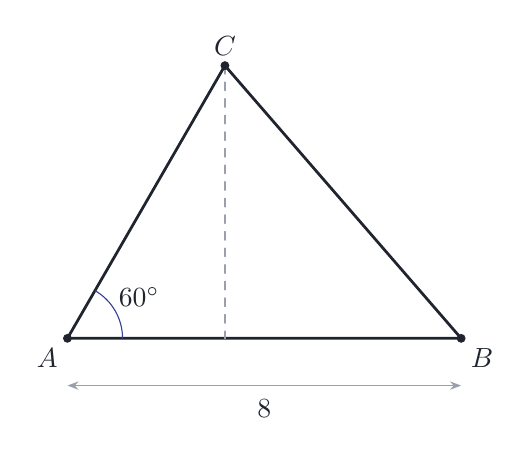
\begin{tikzpicture}

  % ============================================================
  % EJEMPLO 1: triángulo con altura y ángulo (borra y dibuja
  % tu figura; las medidas deben ser geométricamente reales).
  % ============================================================
  \coordinate (A) at (0,0);
  \coordinate (B) at (5,0);
  \coordinate (C) at (2,3.464);   % ángulo en A = 60° de verdad
  \coordinate (H) at (2,0);       % pie de la altura

  \draw[figura] (A) -- (B) -- (C) -- cycle;
  \draw[auxiliar] (C) -- (H);
  \pic [draw=azul, text=azul, angle radius=7mm, angle eccentricity=1.5,
        "$60^\circ$"] {angle = B--A--C};

  \node[punto] at (A) {};  \node[below left]  at (A) {$A$};
  \node[punto] at (B) {};  \node[below right] at (B) {$B$};
  \node[punto] at (C) {};  \node[above]       at (C) {$C$};

  \draw[cota] (0,-0.6) -- (5,-0.6);
  \node[below] at (2.5,-0.65) {$8$};

  % ============================================================
  % EJEMPLO 2: ejes y gráfica de función (descomenta para usar)
  % ============================================================
  % \draw[eje] (-0.5,0) -- (5.2,0) node[below] {$x$};
  % \draw[eje] (0,-0.5) -- (0,3.8) node[left]  {$y$};
  % \draw[figura, color=azul]
  %   plot[domain=0.3:4.5, samples=80] (\x, {0.25*(\x-2)^2 + 0.8});
  % \node[punto] at (2,0.8) {};
  % \node[below right] at (2,0.8) {$V$};
  % \draw[auxiliar] (2,0.8) -- (2,0);

\end{tikzpicture}
\end{document}
